\section{Semantische (Web-)services}
\label{l:sem-web-ser}
\subsection{Einführung}

Anwendungen in Unternehmen werden heute im Gegensatz zu den isolierten Einzellösungen
der Vergangenheitmeist als Aggregate weitgehend eigenständiger Softwarekomponenten realisiert.
Dienstorientierte Architekturen sind die Basis für die Erweiterung dieser Aggregate um
extern erbrachte Dienstkomponenten, die bevorzugt über das Internet als Web Services eingebunden
werden. Damit wird es beispielweise möglich, betriebswirtschaftliche Anwendungen zu
Ablaufketten zu verbinden, externe Informationsdienste in die eigene Planungssoftware einzubeziehen
oder ein netzweites Single-Sign-On zu nutzen. Solche dienstorientierten Architekturen
finden heute große Aufmerksamkeit, weil sich die Anwender dadurch Flexibilität, Interoperabilität,
Anpassungsfähigkeit, Wiederverwendbarkeit, Herstellerunabhängigkeit und letztendlich
Kostenersparnisse für die Entwicklung und den Betrieb der Geschäftsanwendungen erhoffen. \cite{addo}

Web services generalize the idea of the Web beyond the exchange of simple Web pages in order to enable the provision of a broad range of different services. By composing Web services, cross-organizational and collaborative business processes can be realized in a highly dynamic and flexible way, which is particularly important if services have to be automatically procured at runtime. However, achieving a higher degree of automation is obstructed by the informal nature of legal, contractual and organizational regulations, the numerous and complex service descriptions including manifold customization possibilitiesm and the open and heterogeneous nature of the Web service market.

Because many consider them a server-side activity, the
current development of Web services isn’t requester oriented.
Each service provider has its own business logic and
system design.When the service provider upgrades its system
and architecture to improve the service or add new
service functions, service requesters must change their
applications accordingly. For example, the first version of
ArcWeb Services had no point data type.The location data
type contains the x and y values directly. In the second and
third versions, an application must derive the x and y coordinate
values from the point-object data type. Semantics
become a problem because when providers develop services,
they’re more concerned with the business logic and
how to build the service in OOP.This focus concentrates
on syntactic architecture for service development, not
meaning. Afterward, people find it difficult to have
requesters understand and use services without information
about the underlying meaning behind the services by
reading the WSDL document, the product of OOP. \cite{shi1}

The current Web service technology brought a new potential
to the Web of services. However, the success of Web
services still depends on resolving three fundamental challenges,
namely search, integration and mediation. \cite{WSMOLITE}

Was bleibt ist das Problem der Semantik der auszutauschenden Daten. Deswegen denke ich: Öffentliche Service-Verzeichnisse werden sich im Business-Alltag mangels semantischer Standards vorerst nicht durchsetzen. Viel wahrscheinlicher ist zunächst die Migration bestehender Unternehmensverbände (z.B. Zulieferer - Hersteller, etc.) auf eine Service-orientierte Plattform mit einem gemeinsamen privaten Service-Verzeichnis. Dieses wäre ein weiterer Schritt in Richtung der Vision eines Semantic Web Services bzw. dem Semantic Web.  \cite{hhxmlwssoa} 

Such an approach means service providers handle serialization
and deserialization themselves in the knowledge
engineering process, as Figure 3 shows, rather than using
the computer to do it automatically.So, the service description
becomes meaningful as well as independent of the
OOP development.
Because service semantics can remain consistent for long
periods—despite the changes in system design, business
logic, and APIs—publishing requester-oriented service
semantics is better than publishing the changing APIs specified
in WSDL documents. Most Web service users, including
scientists and engineers, aren’t programmers, so
implementing such requester-oriented service design will
let most users exploit distributed computing’s power without
writing a computer program. \cite{shi1}

\begin{figure}
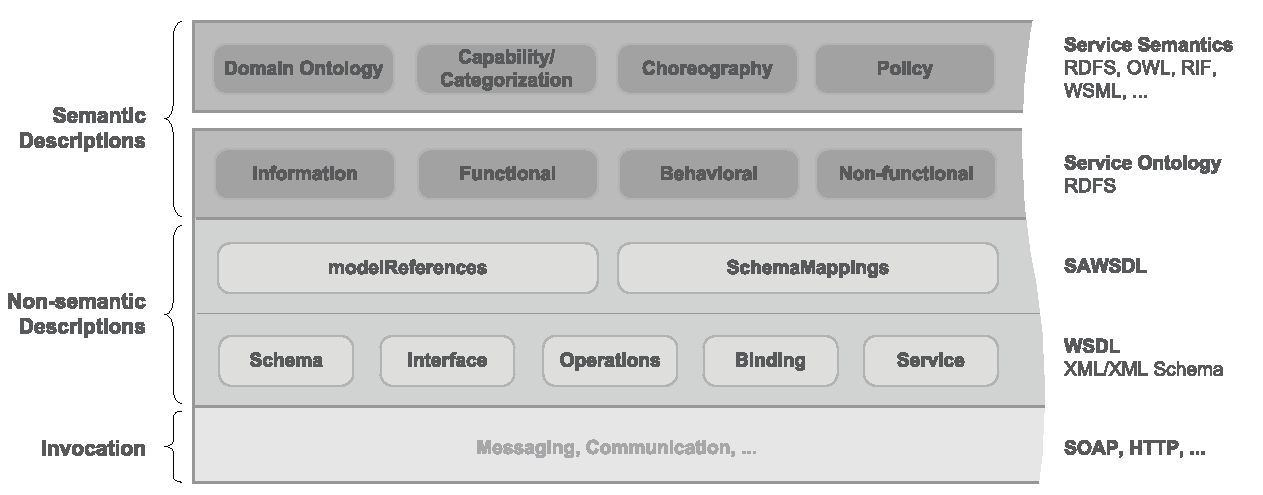
\includegraphics[width=14cm]{media/Extended-Web-Service-Specification-Stack.pdf}
\caption{Extended Web Service Specification Stack, \cite{WSMOLITE}}
\end{figure}

\subsection{Theorie}

% Ontologien etc.

Das Transportieren von Bedeutung ist Ziel jeder Kommunikation. Dabei
differieren oftmals die gedanklichen Verknüpfungen der verwendeten Worte bei
Sender und Empfänger. In Standard-Situationen, wie zum Beispiel beim
Überqueren einer Fußgängerampel oder in anderen stark reglementierten
Abläufen, besteht kaum Klärungsbedarf hinsichtlich der verwendeten Zeichen
oder des verwendeten Vokabulars. Treffen allerdings Sender und Empfänger in
einem weniger stark reglementierten oder unterschiedliche interpretierbarem
Kontext aufeinander, so müssen zuerst das unterschiedlich verwendete Vokabular
und die dahinterstehenden Bedeutungen abgeglichen werden. [und weiter...] \cite{sgthesis}
